\documentclass{article}

% if you need to pass options to natbib, use, e.g.:
% \PassOptionsToPackage{numbers, compress}{natbib}
% before loading nips_2016
%
% to avoid loading the natbib package, add option nonatbib:
% \usepackage[nonatbib]{nips_2016}

% \usepackage{nips_2016}

% to compile a camera-ready version, add the [final] option, e.g.:
\usepackage[final]{nips_2016}
\usepackage{graphicx}
\usepackage{caption}
\usepackage{subcaption}

\usepackage[utf8]{inputenc} % allow utf-8 input
\usepackage[T1]{fontenc}    % use 8-bit T1 fonts
\usepackage{hyperref}       % hyperlinks
\usepackage{url}            % simple URL typesetting
\usepackage{booktabs}       % professional-quality tables
\usepackage{amsfonts}       % blackboard math symbols
\usepackage{nicefrac}       % compact symbols for 1/2, etc.
\usepackage{microtype}      % microtypography


\title{Reinforcement Learning for Chatbot with Emotions}

% The \author macro works with any number of authors. There are two
% commands used to separate the names and addresses of multiple
% authors: \And and \AND.
%
% Using \And between authors leaves it to LaTeX to determine where to
% break the lines. Using \AND forces a line break at that point. So,
% if LaTeX puts 3 of 4 authors names on the first line, and the last
% on the second line, try using \AND instead of \And before the third
% author name.

\author{
  Luyi Ma \\
  School of Computer Science\\
  Carnegie Mellon University\\
  Pittsburgh, PA 15213 \\
  \texttt{luyim@andrew.cmu.edu} \\
  \And
  Zhefan Zhu \\
  School of Computer Science \\
  Carnegie Mellon University\\
  Pittsburgh, PA 15213 \\
  \texttt{zhefanz@andrew.cmu.edu} \\  
  %% examples of more authors
  %% \And
  %% Coauthor \\
  %% Affiliation \\
  %% Address \\
  %% \texttt{email} \\
  %% \AND
  %% Coauthor \\
  %% Affiliation \\
  %% Address \\
  %% \texttt{email} \\
  %% \And
  %% Coauthor \\
  %% Affiliation \\
  %% Address \\
  %% \texttt{email} \\
  %% \And
  %% Coauthor \\
  %% Affiliation \\
  %% Address \\
  %% \texttt{email} \\
}

\begin{document}
% \nipsfinalcopy is no longer used

\maketitle






\section{Background}

Dialogue systems, such as chatbots have become ubiquitous in modern society. A lot of chatbots have been presented so far. One of the latest chatbots is MILABOT, which is based on deep reinforcement learning, and developed by the Montreal Institute for Learning Algorithms (Serban, Sankar et al. 2017). Figure \ref{fig:dialoguesystem} shows their system control flow. In their chatbot, they have several response models to generate response separately to the input sentence, and the system is also given the dialogue history. The responses generated by sub-models are selected and evaluated according to some selection policies, and the best response is returned to the user. \par 





\begin{figure}[!h]
\begin{center}
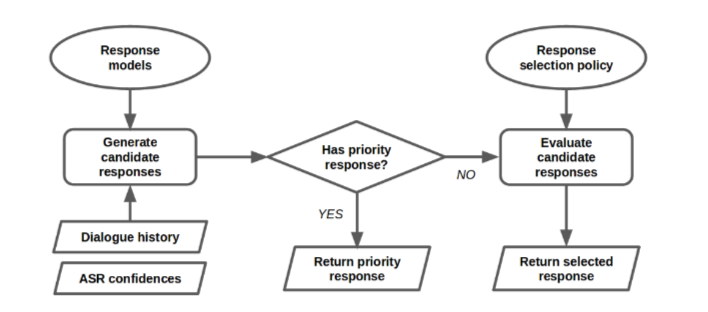
\includegraphics[scale=0.4]{figure1.png}
\caption{Dialogue manager control flow.}
\label{fig:dialoguesystem}
\end{center}
\end{figure}


The essential part of a dialogue system is response models. Common response models include knowledge based Q\&A systems, template based models, retrieval based neural networks, and generation based neural networks. \par



For our goal setting, we mainly focus on generation based neural networks. One typical model is the encoder-decoder framework of seq2seq model (Zhou, et al. 2017), where both layers are GRU layers (cho et al. 2014). In this framework, the encoder layer converts input sequence $X = (x_1, x_2, ..., x_n)$ to hidden state $h = (h_1, h_2, ..., h_n)$. And for the decoder layer, it takes in a context vector and previously decoded word to generate its state $s_t$. The output token is generated by sampling from output probability distribution computed by $s_t$.




\section{Data and Method}

\subsection{Dataset and Preprocessing}

To train the response model, we collected 2.7 million sentences of subtitles from open subtitle database (\url{http://opus.lingfil.uu.se/OpenSubtitles.php/}). We choose subtitle dataset, because it is difficult to obtain chatting dataset, and subtitles are pretty similar to dalogues at most of the time. The subtitles of movies and TV programs provide sufficient conversation contents for training. Nevertheless, subtitles are slightly different from daily conversation due to theatrical and dramatic contents. We parsed conversations from original data which was in .xml format, and filtered long segment of words which is impractical in daily conversation, which could be monologues in movies. \par

To train the model determining the emotion of a sentence, we used a dataset of tweets with emotion labels from http://knoesis.org/library/resource.php?id=1749 (Wang et al. 2012). This dataset tags tweets with seven emotions: anger, fear, joy, love, sadness, surprise and thankfulness. The format of the original dataset is: tweetId TAB emotionTag. We implemented a crawler to query tweet content from websites and constructed the training set. \par 

In addition, the word2seq embedding vectors (50 dimensions) are obtained from GloVe (https://nlp.stanford.edu/projects/glove/), which is used to transform words into vectors. 















\section{Experiments \& Results}
\subsection{Tweet classification}

We trained the simple LSTM model with 80\% of the total tweet dataset, and used remaining 20\% for evaluating the model performance. Since every sample tweet has different length of words, the batch size of the model is set to 1, and figure \ref{fig:test error} shows the trend of test classification error vs. number of training samples. The model converges very fast, and achieves minimum testing error after 20000 iterations (tweet samples). Table \ref{sentence} shows the prediction results of some sentences picked randomly from websites. We can notice that our model tends to give positive predictions to the inputs, which requires further study. 




\begin{figure}
\begin{center}
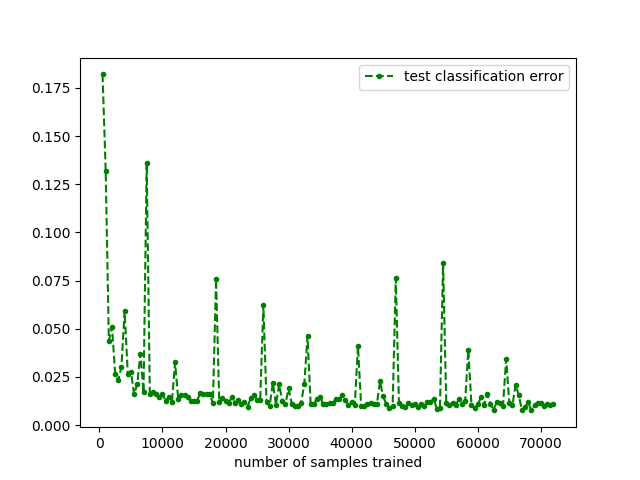
\includegraphics[scale=0.6]{Figure2.png}
\caption{Test classification error of simple LSTM model.}
\label{fig:test error}
\end{center}
\end{figure}


\begin{table}[tbp]
\centering  % 表居中
\begin{tabular}{lccc}  % {lccc} 表示各列元素对齐方式,left-l,right-r,center-c
\hline
Sentence &Predicted emotion &True emotion\\ \hline  % \hline 在此行下面画一横线
I so pissed . Roger just stabbed me in the back . &joy &anger \\         % \\ 表示重新开始一行
I so frustrated . &sadness &sadness \\        % & 表示列的分隔线
It's so frustrating working with him . &love &anger\\ 
I was so frustrated , I stopped caring about the outcome . &fear &anger \\
I feeling pretty good right now . &joy &joy \\
I in a very good mood . &fear &joy \\
It feels so good taking a long vacation . &joy &joy \\
I got everything I ever wanted. I feel so blessed . &joy &joy \\ \hline
\end{tabular}
\caption{Predictions of some random sentences.}
\label{sentence}
\end{table}




















\section*{References}

[1] Cho, K., Van Merriënboer, B., Bahdanau, D., \& Bengio, Y. (2014). On the properties of neural machine translation: Encoder-decoder approaches. arXiv preprint arXiv:1409.1259.


[2] Serban, I. V., Sankar, C., Germain, M., Zhang, S., Lin, Z., Subramanian, S., ... \& Mudumba, S. (2017). A Deep Reinforcement Learning Chatbot. arXiv preprint arXiv:1709.02349.

[3] Wang, W., Chen, L., Thirunarayan, K., \& Sheth, A. P. (2012, September). Harnessing twitter" big data" for automatic emotion identification. In Privacy, Security, Risk and Trust (PASSAT), 2012 International Conference on and 2012 International Confernece on Social Computing (SocialCom) (pp. 587-592). IEEE.

[4] Zhou, H., Huang, M., Zhang, T., Zhu, X., \& Liu, B. (2017). Emotional Chatting Machine: Emotional Conversation Generation with Internal and External Memory. arXiv preprint arXiv:1704.01074.
\end{document}
